\documentclass[12pt, a4paper]{article}

\usepackage{gset} 
\usepackage{preamble}
\usepackage{accents}
\newtheorem{theorem}{Теорема}
\newtheorem{lemm}{Лемма}

\begin{document}
{\textbf{\large Матанализ}\hfill \textbf{(Основной поток)}
	
	\medskip %
	
	\textbf{Домашнее задание 12}}

\medskip

\p Найти промежутки монотонности, точки локальных и глобальных экстремумов

\sp $f(x) = \dfrac{3x - 7}{(x^2 - 1)^2}$

$f'(x) = \dfrac{3(x^2 - 1)^2 - (3x - 7)(x^2 - 1)*4x}{(x^2 - 1)^4}$

Найдем точки, в которых $f'(x) = 0$: 

$3(x^2 - 1)^2 - (3x - 7)(x^2 - 1) * 4x = 0$

$(x^2 - 1)(3(x^2 - 1) - (3x - 7) * 4x) = 0$

$x = \pm 1$

или 

$9x^2 + 28x - 3 = 0$

$x \in \{-1, \dfrac{1}{9}, 1, 3\}$

\[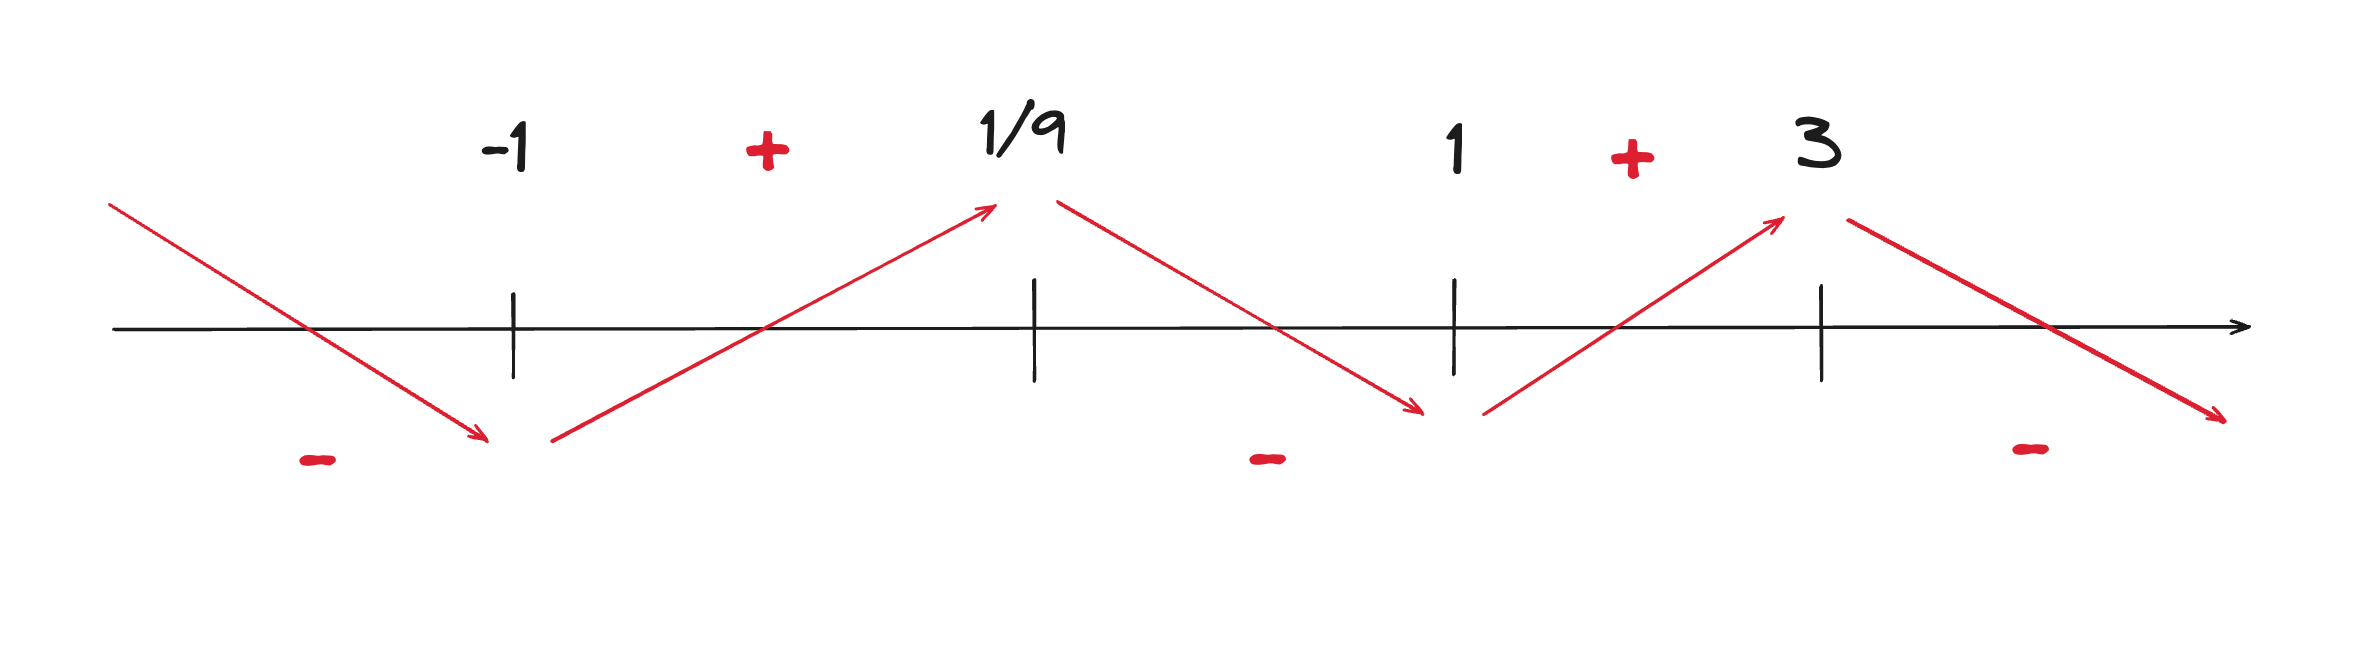
\includegraphics[width=150mm]{img}\] 

$L min$: не существует, так как $\pm 1$ не входит в область определения

$L max$: $x = \dfrac{1}{9}$, $x = 3$. 

$G min$: не существует

$G max$: нужно сравнить $f(\dfrac{1}{9})$, $f(3)$, $\lim\limits_{x \to -\infty} f(x)$ 

$f(\dfrac{1}{9}) = -\dfrac{2187}{320}$\quad
$f(3) = \dfrac{1}{32}$\quad
$\lim\limits_{x \to \infty} f(x) = 0$

$G max$: $x = 3$\\

\sp $f(x) = \begin{cases}
	x^{xlnx}, &\text{ если }x > 0\\
	1, &\text{ если } x = 0  
\end{cases}$

$(x^{xlnx})' = e^{xln^2x} = e^{xln^2x} * (xln^2x)' = e^{xln^2x}  * (ln^2x + 2lnx)$

$f'(x) = \begin{cases}
	e^{xln^2x}  * (ln^2x + 2lnx), &\text{ если }x > 0\\	
	0, &\text{ если } x = 0\\
\end{cases}$

Найдем точки, в которых $f'(x) = 0$

$x = 0$

или 

$ln^2x + 2lnx = 0$

$lnx(lnx + 2) = 0$

$lnx = 0 $ или $lnx = - 2$

$x = 1$ или $x = e^{-2}$

$x \in \{0, e^{-2}, 1\}$

\[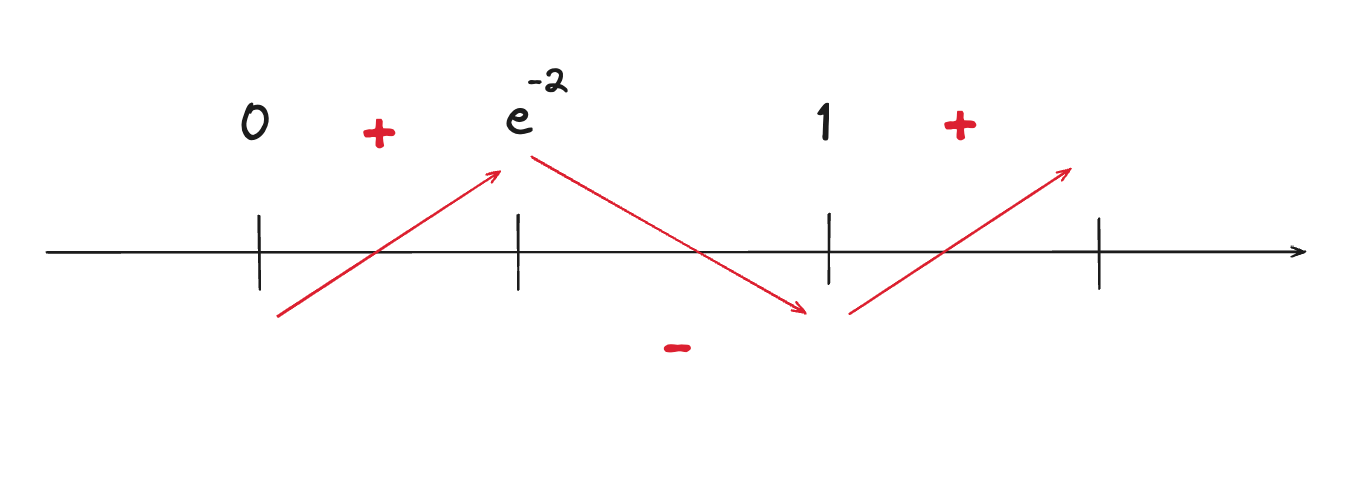
\includegraphics[width=150mm]{img1}\]

$L min$: $x = 1$

$L max$: $x = e^{-2}$. 

$G min$: нужно сравнить $f(0), f(1)$

$f(0) = 1$

$f(1) = 1$

$G min$: $x = 1$

$G max$: нужно сравнить $f(e^{-2}), \lim\limits_{x \to \infty} f(x)$ 

$f(e^{-2}) = e^{4e^{-2}}$ \quad
$\lim\limits_{x \to \infty} f(x) = \infty$

$G max$: не существует

\p Для функции $f(x) = \begin{cases}
	sinx, &\text{ если } x \geq 0\\
	x^2, &\text{ если } x < 0
	\end{cases}$

\sp найти прожутки монотонности, точки локальных и глобальных экстремумов

$f'(x) = \begin{cases}
	cosx, &\text{ если }x \geq 0\\	
	2x, &\text{ если }x < 0\\
\end{cases}$

Найдем точки, в которых $f'(x) = 0$

$cosx = 0, x \geq 0$

или 

$2x = 0, x < 0$

$x \in \dfrac{\pi}{2} + \pi k, k \in \N$

Так как функция периодичная, рассмотрим только первый период $[0, 2\pi]$

\[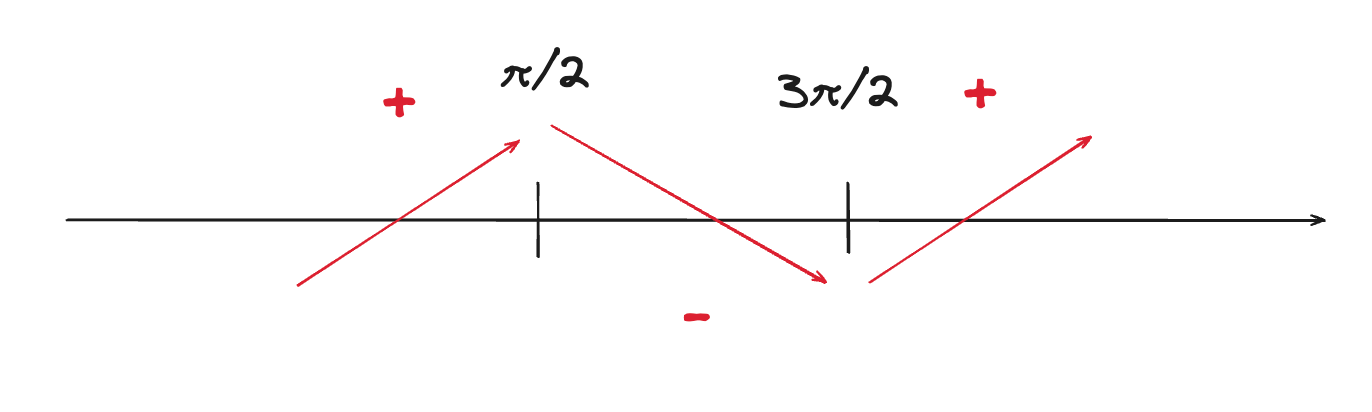
\includegraphics[width=150mm]{img2}\]

$Lmin$: $\dfrac{3\pi}{2} + 2\pi k, k \in \N$

$Lmax$: $\dfrac{\pi}{2} + 2\pi k, k \in \N$

$Gmin$: $\dfrac{3\pi}{2} + 2\pi k, k \in \N$

$Gmax$: $\dfrac{\pi}{2} + 2\pi k, k \in \N$

\sp найти промежутки, на которых функция является выпуклой, вогнутой

$f''(x) = \begin{cases}
	-sinx, &\text{ если }x \geq 0\\	
	2, &\text{ если }x < 0
\end{cases}$

$-sinx = 0, x \geq 0$

$x \in \pi k, k \in \N$

Опять рассмотрим только один период $[\dfrac{\pi}{2}, \dfrac{5\pi}{2}]$

\[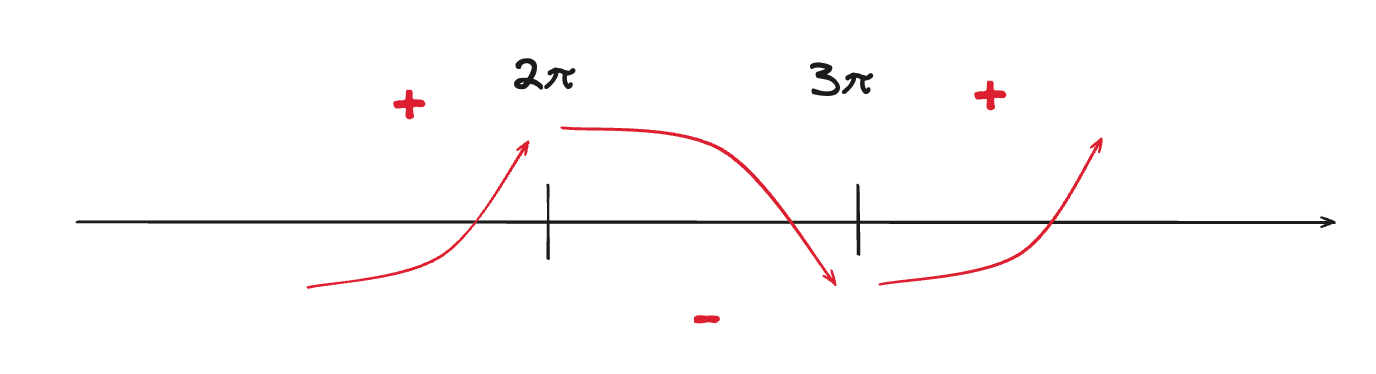
\includegraphics[width=150mm]{img3}\]

Функция выпуклая на промежутках $[\pi + 2\pi k, 2\pi + 2\pi k], k \in \N$

Функция вогнутая на промежутках $[2\pi k, \pi + 2\pi k], k \in \N$
\\ 

\p Доказать неравенства 

\sp $1 + \dfrac{x}{2} - \dfrac{x^2}{8} < \sqrt{1 + x} < 1 + \dfrac{x}{2} \quad,  \forall x > 0$ 

Докажем $1 + \dfrac{x}{2} - \dfrac{x^2}{8} < \sqrt{1 + x}$

$g(x) = \sqrt{1 + x} - 1 - \dfrac{x}{2} + \dfrac{x^2}{8}$

$g'(x) = \dfrac{1}{2\sqrt{1 + x}} - \dfrac{1}{2} + \dfrac{x}{4}$

Разложим по Формуле 1 при $n = 0, \lambda = 0 $

$\sqrt{1 + x} - 1 - \dfrac{x}{2} + \dfrac{x^2}{8} = g(0) + g'(c) = 0 + \dfrac{1}{2\sqrt{1 + c}} - \dfrac{1}{2} + \dfrac{c}{4}$

Хотим доказать, что $\dfrac{1}{2\sqrt{1 + c}} - \dfrac{1}{2} + \dfrac{c}{4} > 0, \forall c > 0$

$f(c) = \dfrac{1}{2\sqrt{1 + c}} - \dfrac{1}{2} + \dfrac{c}{4}$

$f'(c) = \dfrac{1}{4} - (2\sqrt{1 + c})^{-2}$

$f'(c) = 0$ при $c = 0$

То есть при $c \in $ $(0, +\infty] f(x) > f(0) = 0$

Докажем $\sqrt{1 + x} < 1 + \dfrac{x}{2}$ 

$f(x) = 1 + \dfrac{x}{2} - \sqrt{1 + x}$ 

$f'(x)$

Разложим по Формуле 1 при $n = 0$, $\lambda = 0$

$1 + \dfrac{x}{2} - \sqrt{1 + x} = 0 + x(\dfrac{1}{2} - \dfrac{1}{2(1 + c))}$

$c > 0 \Rightarrow \dfrac{1}{2} > \dfrac{1}{2(1 + c)}$

$\begin{cases}
	x > 0\\
	\dfrac{1}{2} > \dfrac{1}{2(1 + c)}
\end{cases} \Rightarrow \sqrt{1 + x} < 1 + \dfrac{x}{2}$

\sp $\dfrac{b - a}{b} < ln \dfrac{b}{a} < \dfrac{b - a}{a} \quad , \forall 0 < a < b$

Докажем $ln \dfrac{b}{a} < \dfrac{b - a}{a}$

$\forall x > 0: e^x > 1 + x \Rightarrow x > ln(1 + x)$

Пусть $1 + x = \dfrac{b}{a}, x = \dfrac{b - a}{a}, ln(1 + x) = ln\dfrac{b}{a}$

$x > ln(1 + x) \Rightarrow \dfrac{b - a}{a} > ln\dfrac{b}{a}$

Докажем $\dfrac{b - a}{b} < ln \dfrac{b}{a}$

$x > ln(1 + x) \Rightarrow -x < -ln(1 + x) \Rightarrow -x < ln(\dfrac{1}{1 + x}) $

Пусть $1 + x = \dfrac{a}{b}, x = \dfrac{a - b}{b}, -x = \dfrac{b - a}{b}, ln(1 + x) = ln(\dfrac{a}{b}), ln(\dfrac{1}{1 + x}) = ln(\dfrac{b}{a})$

$-x < ln(\dfrac{1}{1 + x}) \Rightarrow \dfrac{b - a}{b} < ln(\dfrac{b}{a})$

\p Доказать утверждения 

\sp Если $x, y, z > 0, x + y + z = 3\pi$, то $x^x + y^y + z^z > 108$

Используем неравенство Йенсена при $n = 3, \lambda_i = \dfrac{1}{3}, f(x) = x^x$

Определим выпуклость $f(x)$

$(x^x)' = (e^{xlnx})' = x^x (lnx + 1)$

$(x^x)'' = (x^x (lnx + 1))' = (x^x)'(lnx + 1) + x^x(lnx + 1)' = x^x(lnx + 1)^2 + x^{x - 1} > 0 \forall x \geq 0$

$f(x) -$ выпуклая

$36 < \pi^\pi \leq \dfrac{x^x + y^y + z^z}{3} \Rightarrow x^x + y^y + z^z> 3 * 36 = 108$

\sp $\sqrt[n]{x_1x_2\cdots x_n} \leq \dfrac{x_1 + x_2 + \cdots + x_n}{n}$

Используем неравенство Йенсена при $n = n, \lambda_i = \dfrac{1}{n}, f(x) = lnx$

Определим выпуклость $f(x)$

$f'(x) = \dfrac{1}{x}$

$f''(x) = -\dfrac{1}{x^2} < 0 - $ $f(x) $вогнутая

$ln(\dfrac{x_1 + x_2 + \cdots + x_n}{n}) \geq \dfrac{ln(x_1*x_2*\cdots*x_n)}{n}$

$ln(\dfrac{x_1 + x_2 + \cdots + x_n}{n}) \geq ln(\sqrt[n]{x_1*x_2*\cdots*x_n})$

$\dfrac{x_1 + x_2 + \cdots + x_n}{n} \geq \sqrt[n]{x_1*x_2*\cdots*x_n}$


\p Найти максимальную сумму $sinA + sinB + sinC,$ где $A + B + C = 180, A, B, C \in [0, \pi]$

Используем неравенство Йенсена при $n = 3, \lambda_i = \dfrac{1}{n}, f(x) = sinx, f''(x) = -sinx < 0 $ - вогнутая на $[0, \pi]$

$sin\dfrac{\pi}{3} \geq \dfrac{sinA + sinB + sinC}{3} \Rightarrow sinA + sinB + sinC \leq 3 * \dfrac{\sqrt{3}}{2}$

\end{document}
